\chapter{Free energy calculation}

\vspace{-1cm} \noindent \textcolor{graytitle}{\textit{{\Large Simple sampling of a free energy barrier using umbrella sampling}}\vspace{0.5cm} }

\noindent \hspace{-0.45cm}\begin{wrapfigure}{r}{4cm}
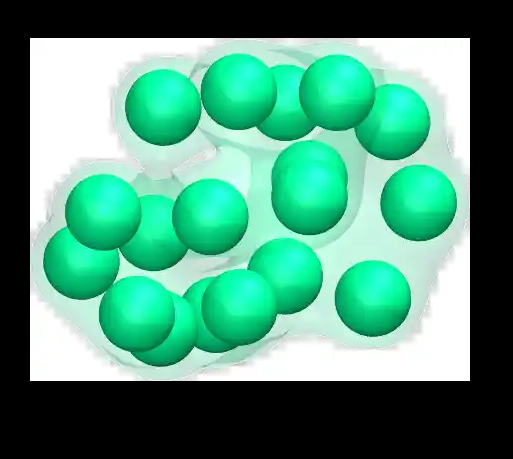
\includegraphics[width=4cm]{tutorials/level3/free-energy-calculation/avatar_light.png}
\end{wrapfigure}

\noindent The objective of this tutorial is to measure the free
energy profile across a barrier potential using two methods;
:ref:`free sampling <method1>` and :ref:`umbrella sampling <method2>`.

For the sake of simplicity and in order to reduce the computation time, the
barrier potential will be imposed artificially to the atoms.
The procedure is valid for more complex
systems, and can be adapted to many other situations, for instance 
for measuring adsorption barrier near a wall, or for calculating translocation
barrier through a membrane.

\section{Method 1: Free sampling}

\noindent The most direct way to calculate a free energy profile is to extract
the partition function from a classic (unbiased) molecular
dynamics simulation, and then to estimate the Gibbs free
energy using 

where $\Delta G$ is the free energy difference, R the
gas constant, T the temperature, p the
pressure, and $p_0$ the reference pressure.
As an illustration, let us apply this method to an
extremely simple configuration that consists in a few
particles diffusing in a box in presence of a
position-dependent repealing force that makes the centre
of the box a relatively unfavourable area to explore.

\subsection{Basic LAMMPS parameters}

\noindent Create a folder named \textit{FreeSampling/}, and create an input script
named \textit{input.lammps} in it. Copy the following lines:

\begin{lcverbatim}
# define some variables
variable sigma equal 3.405 # Angstrom
variable epsilon equal 0.238 # Kcal/mol
variable U0 equal 1.5*${epsilon} # Kcal/mol
variable dlt equal 1.0 # Angstrom
variable x0 equal 10.0  # Angstrom
# initialise the simulation
units real
atom_style atomic
pair_style lj/cut 3.822 # 2^(1/6) * 3.405 WCA potential
pair_modify shift yes
boundary p p p
\end{lcverbatim}

\noindent Here, we start by defining variables for the Lennard-Jones
interaction $\sigma$ and $\epsilon$ and for
the repulsive potential $U (x)$: $U_0$, $\delta$, and $x_0$, 
see the analytical expression below.
The system of unit 'real' (for which energy is in kcal/mol, distance in Ångstrom,
time in femtosecond) has been chosen for practical reason,
as the WHAM algorithm we are going to use in the second
part of the tutorial automatically assumes the energy to
be in kcal/mol. Atoms will interact through a
Lennard-Jones potential with a cut-off equal to 
$\sigma \times 2 ^ {1/6}$ (i.e. a WCA repulsive
potential). The potential is shifted to be equal to 0 at
the cut-off using the \textit{pair$\_$modify}.

\subsection{System creation and settings}

\noindent Let us define the simulation block and randomly add atoms:

\begin{lcverbatim}
# define the system
region myreg block -25 25 -5 5 -25 25
create_box 1 myreg
create_atoms 1 random 60 341341 myreg overlap 1.0 maxtry 50
# settings
mass * 39.95
pair_coeff * * ${epsilon} ${sigma}
neigh_modify every 1 delay 4 check yes
\end{lcverbatim}

\noindent Here I am using the argon's values of the Lennard-Jones parameters $\sigma$ and
$\epsilon$, as well as the mass $m = 39.95$
grams/mole. 

In the previous subsection, the variables $U_0$, $\delta$, and
$x_0$ were defined. They are used to create the repulsive potential
restricting the atoms to explore the center of the box: 

$$U(x) = U_0 \left[ \arctan \left( \dfrac{x+x_0}{\delta} \right) - \arctan \left(\dfrac{x-x_0}{\delta} \right) \right]. $$
From the derivative of the
potential with respect to $x$, we obtain the expression
for the force that will be imposed to the atoms:

$$F(x)= \dfrac{U_0}{\delta} \left[ \dfrac{1}{(x-x_0)^2/\delta^2+1} - \dfrac{1}{(x+x_0)^2/\delta^2+1} \right].$$
The potential and force along the $x$
axis resemble:

\begin{figure}
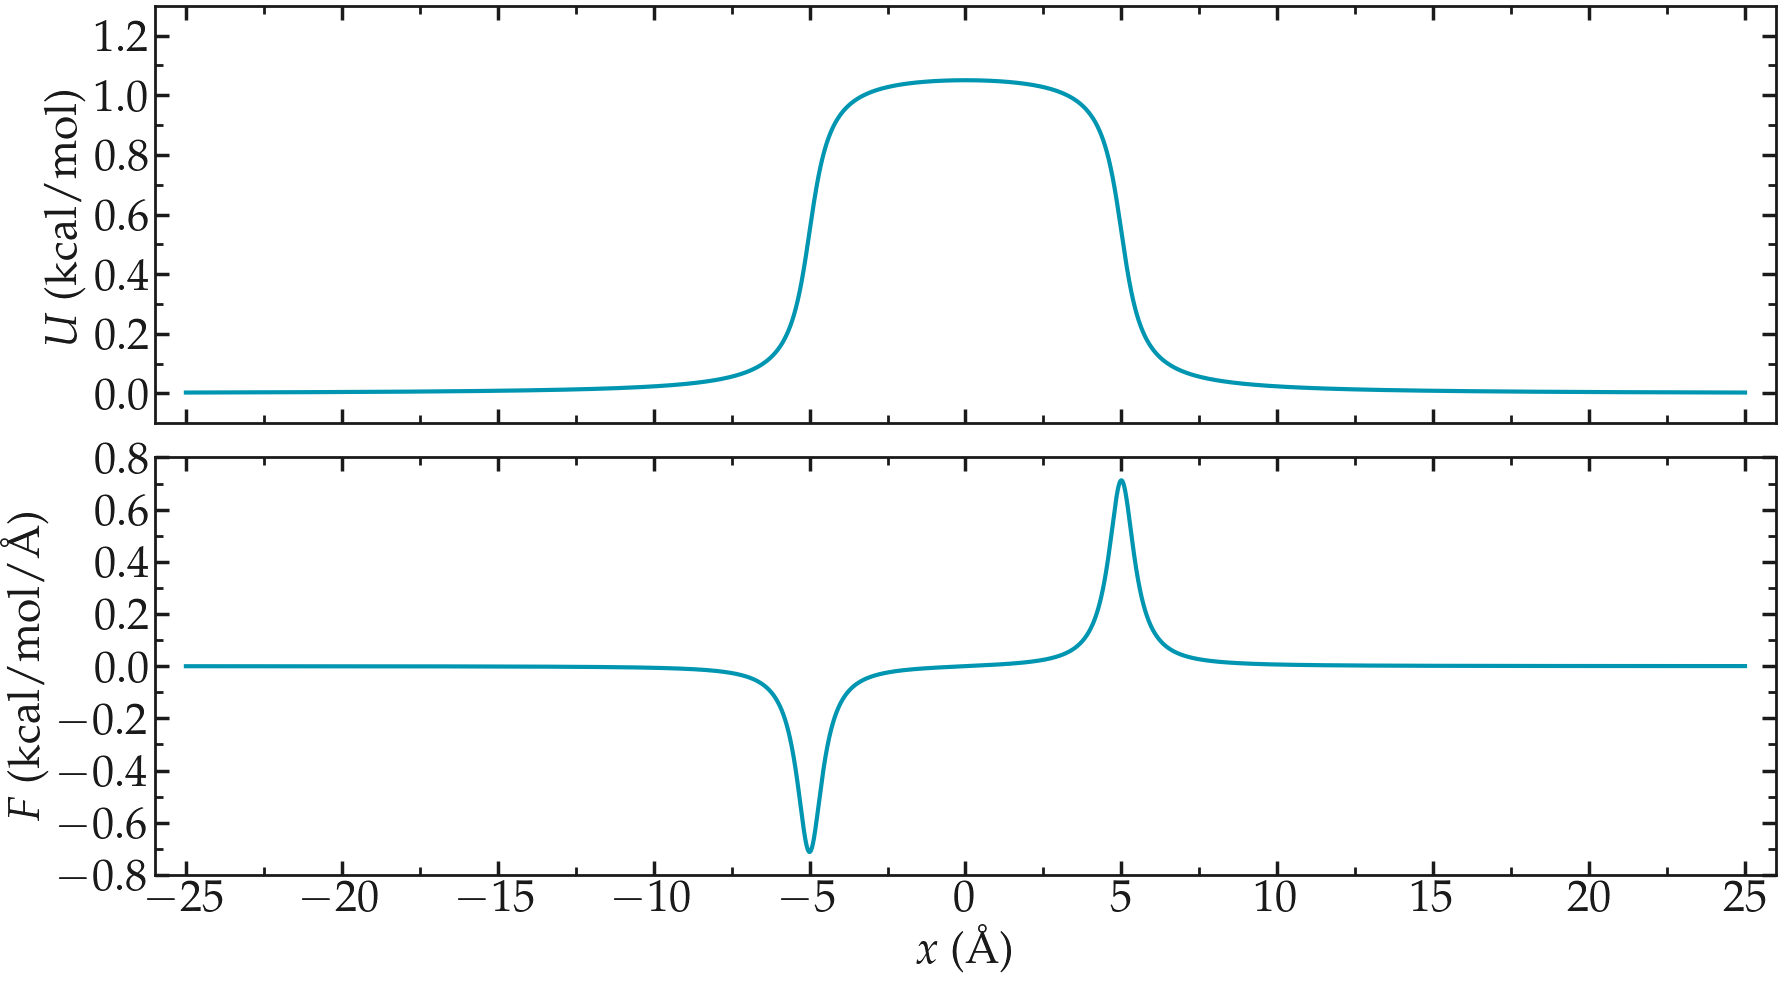
\includegraphics[width=\linewidth]{tutorials/level3/free-energy-calculation/potential-light.png}
\end{figure}

Let us apply energy minimization to the system, and then impose
the force \\(F(x)\\) to all of the atoms in the simulation using the 'addforce' command:

\begin{lcverbatim}
# --------------------- Run
minimize 1e-4 1e-6 100 1000
reset_timestep 0
variable U atom ${U0}*atan((x+${x0})/${dlt})-${U0}*atan((x-${x0})/${dlt})
variable F atom ${U0}/((x-${x0})^2/${dlt}^2+1)/${dlt}-${U0}/((x+${x0})^2/${dlt}^2+1)/${dlt}
fix myadf all addforce v_F 0.0 0.0 energy v_U
\end{lcverbatim}

\noindent Finally, let us combine the fix nve with a Langevin
thermostat to run a molecular dynamics simulation. With
these two commands, the MD simulation is effectively in the
NVT ensemble: constant number of atoms $N$, constant
volume $V$, and constant temperature $T$. Let us
perform an equilibration of 500000 steps in total,
using a timestep of 2 ps (i.e. a total duration of 1
nanoseconds). To make sure that 1 ns is long enough, let us
record the evolution of the number of atoms in the central
(energetically unfavorable) region called \textit{mymes}:

\begin{lcverbatim}
fix mynve all nve
fix mylgv all langevin 119.8 119.8 50 1530917
region mymes block -${x0} ${x0} INF INF INF INF 
variable n_center equal count(all,mymes)
fix myat all ave/time 10 50 500 v_n_center file density_evolution.dat
timestep 2.0
thermo 10000
run 500000
\end{lcverbatim}

\noindent \subsection{Run and data acquisition}

Finally, let us record the density profile of the atoms
along the $x$ axis using the 'ave/chunk' command. A
total of ten density profiles will be printed. Step counts are
reset to 0 to synchronize with the output times of
density/number, and the fix 'myat' is canceled (it has to be
canceled before a reset time).

\begin{lcverbatim}
unfix myat
reset_timestep 0
compute cc1 all chunk/atom bin/1d x 0.0 1.0
fix myac all ave/chunk 10 400000 4000000 cc1 density/number file density_profile_8ns.dat
dump mydmp all atom 200000 dump.lammpstrj
thermo 100000
run 4000000
\end{lcverbatim}

\noindent This simulation with a duration of 8 ns needs a few
minutes to complete. Feel free to increase the 
duration of the run for smoother results.

You can visualize the dump file using VMD:

\begin{figure}
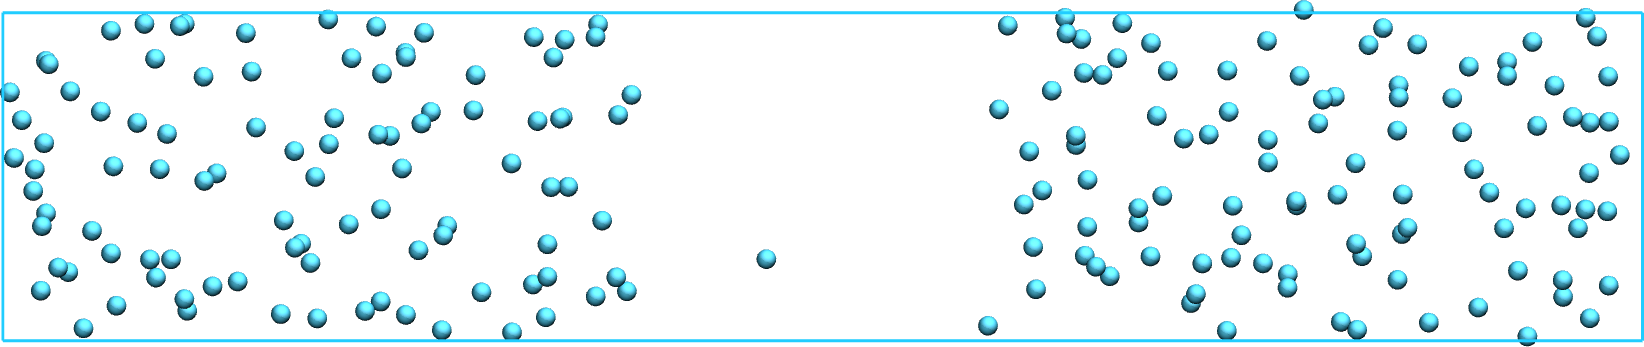
\includegraphics[width=\linewidth]{tutorials/level3/free-energy-calculation/system-light.png}
\end{figure}

\subsection{Data analysis}

\noindent First, let us make sure that the equilibration duration of 1
ns is long enough by looking at the \textit{density$\_$evolution.dat} file:

\begin{figure}
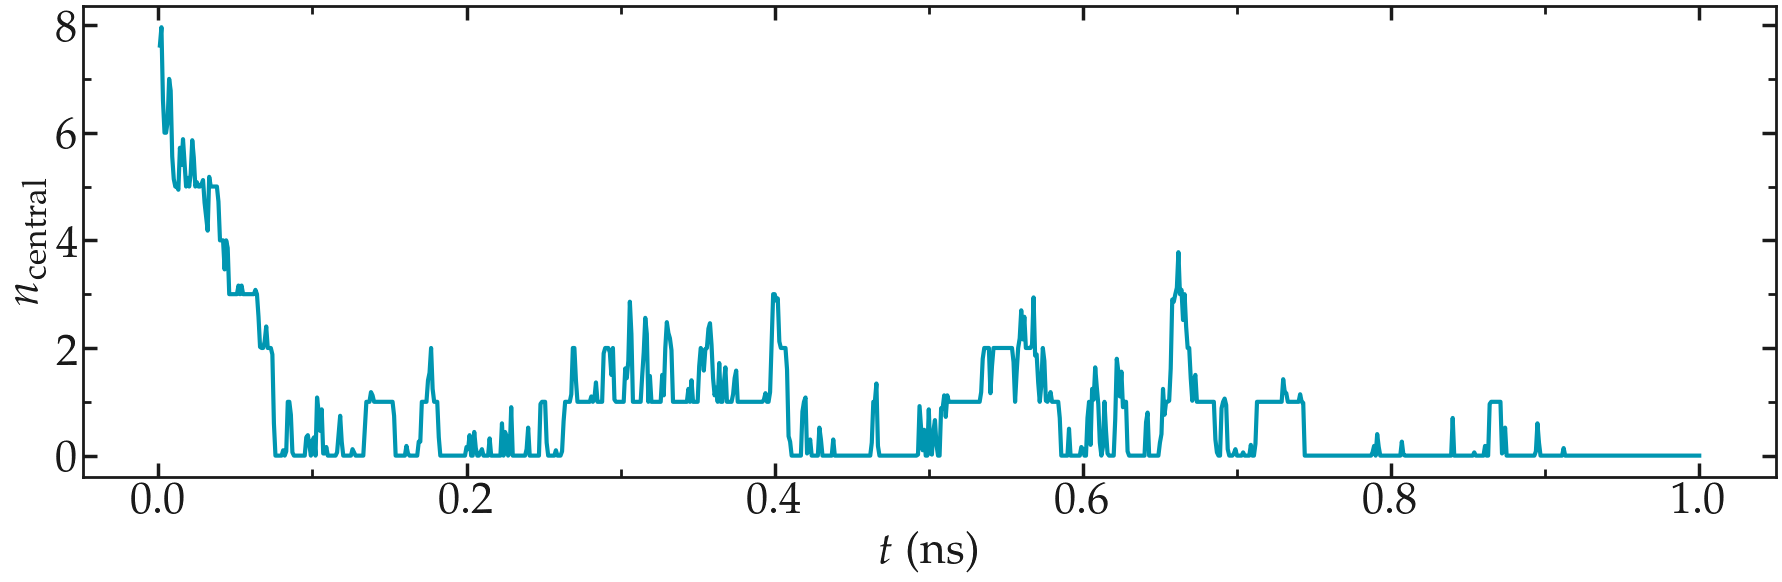
\includegraphics[width=\linewidth]{tutorials/level3/free-energy-calculation/density_evolution-light.png}
\end{figure}

Here, we can clearly see that the number of atoms in the
central region, $n_\mathrm{central}$, evolves to its equilibrium value
after about 0.1 ns.

Let us also plot the equilibrium density profile $\rho$:

\begin{figure}
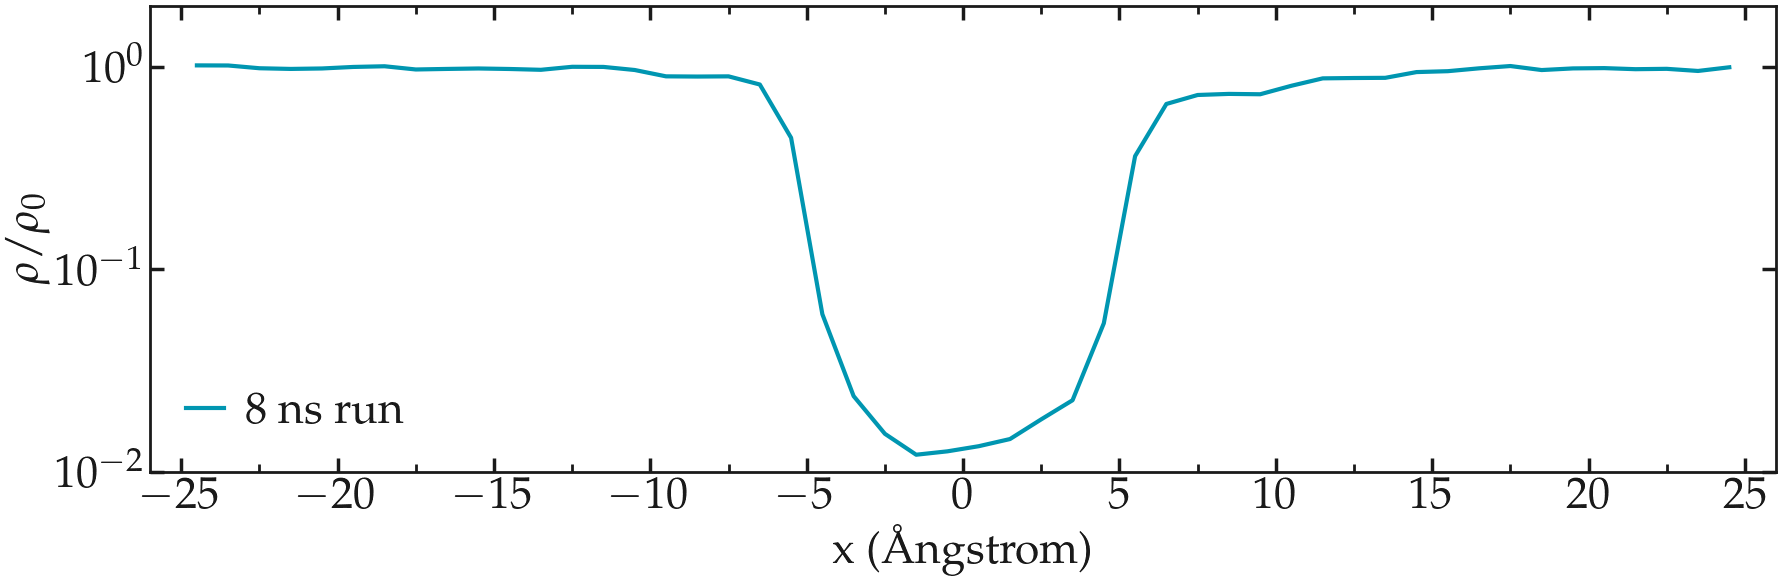
\includegraphics[width=\linewidth]{tutorials/level3/free-energy-calculation/density_profile-light.png}
\end{figure}

Then, let us plot $-R T \ln(\rho/\rho_\mathrm{bulk})$ and compare it
with the imposed (reference) potential $U$:

\begin{figure}
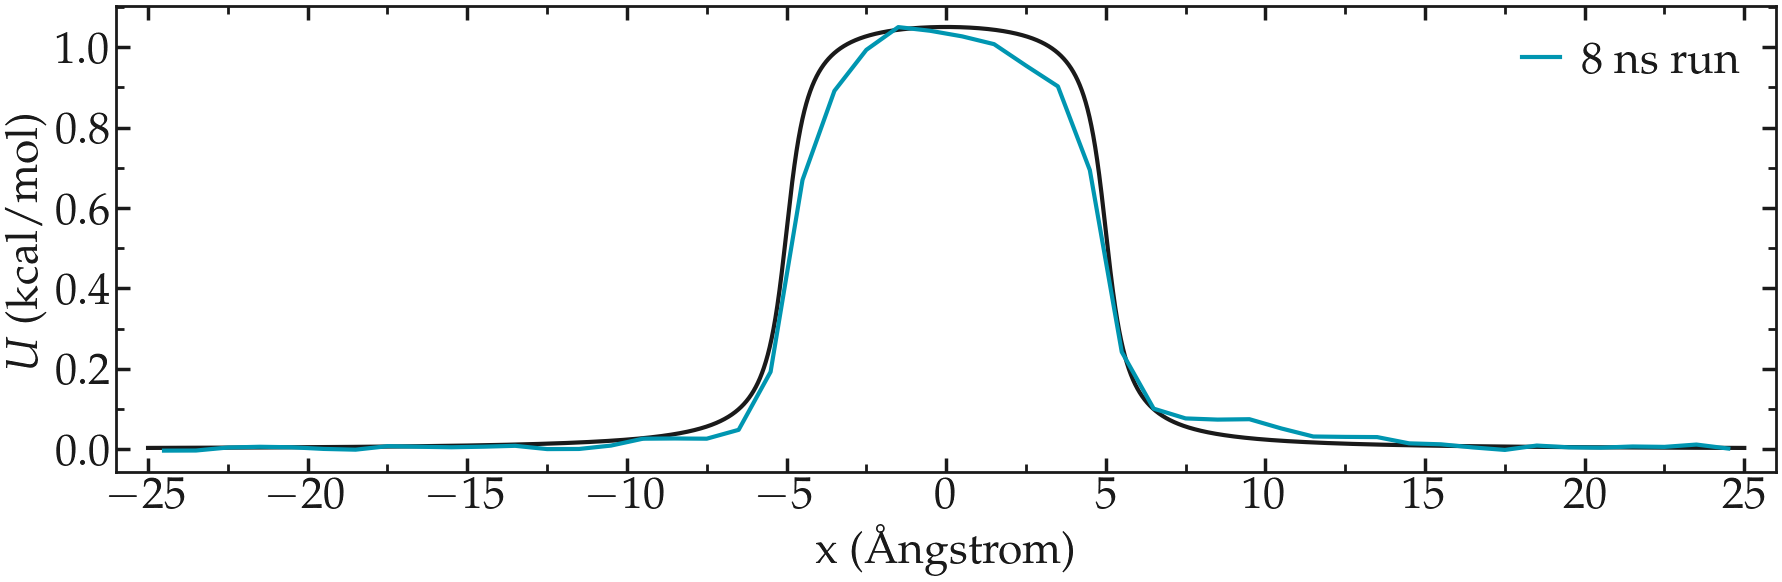
\includegraphics[width=\linewidth]{tutorials/level3/free-energy-calculation/freesampling-potential-light.png}
\end{figure}

The agreement with the expected energy profile is reasonable,
despite some noise in the central part. 

\subsection{The limits of free sampling}

\noindent If we increase the value of $U_0$, the average number of
atoms in the central region will decrease, making it
difficult to obtain a good resolution for the free energy
profile.
In that case, it is better to use the umbrella sampling method
to extract free energy profiles, see the next section.

\section{Method 2: Umbrella sampling}

\noindent Umbrella sampling is a biased molecular dynamics method,
i.e. a method in which additional forces are added to the
atoms in order to make the unfavourable states more likely
to occur.

Keeping the present configuration, we are going to force one of the atom to
explore the central region of the box. To do so, we
are going to add a potential $V$ to one
of the particle, and force it to move along the axe $x$.
The chosen path is called the axe of reaction. The final
simulation will be analyzed using the weighted histogram
analysis method (WHAM), which allows to remove the effect of
the bias and eventually deduce the unbiased free energy profile.

\subsection{LAMMPS input script}

\noindent Create a new folder called \textit{BiasedSampling/}, create a new input file 
named \textit{input.lammps} in it, and copy the following lines:

\begin{lcverbatim}
# define a bunch of variables
variable sigma equal 3.405 # Angstrom
variable epsilon equal 0.238 # Kcal/mol
variable U0 equal 10*${epsilon} # Kcal/mol
variable dlt equal 0.5 # Angstrom
variable x0 equal 5.0  # Angstrom
variable k equal 1.5 # Kcal/mol/Angstrom^2
# initialise the simulation
units real
atom_style atomic
pair_style lj/cut 3.822 # 2^(1/6) * 3.405 WCA potential
pair_modify shift yes
boundary p p p
# define the system
region myreg block -25 25 -5 5 -25 25
create_box 2 myreg
create_atoms 2 single 0 0 0
create_atoms 1 random 5 341341 myreg overlap 1.0 maxtry 50
# settings
mass * 39.948
pair_coeff * * ${epsilon} ${sigma}
neigh_modify every 1 delay 4 check yes
group topull type 2
# run
variable U atom ${U0}*atan((x+${x0})/${dlt})-${U0}*atan((x-${x0})/${dlt})
variable F atom ${U0}/((x-${x0})^2/${dlt}^2+1)/${dlt}-${U0}/((x+${x0})^2/${dlt}^2+1)/${dlt}
fix pot all addforce v_F 0.0 0.0 energy v_U
fix mynve all nve
fix mylgv all langevin 119.8 119.8 50 1530917
timestep 2.0
thermo 100000
run 500000
reset_timestep 0
dump mydmp all atom 1000000 dump.lammpstrj
\end{lcverbatim}

\noindent So far, this code resembles the one of Method 1,
except for the additional particle of type 2. This
particle is identical to the particles of type 1 (same
mass and Lennard-Jones parameters), but will be exposed to the
biasing potential.
The value of the potential $U_0$ was chosen to be much larger than in part 1, 
just to proof that umbrella sampling can easily deal with huge potential value,
while free sampling couldn't.
Let us create a loop with 50 steps, and move progressively
the centre of the bias potential by increment of 0.1 nm:

\begin{lcverbatim}
variable a loop 50
label loop
variable xdes equal ${a}-25
variable xave equal xcm(topull,x)
fix mytth topull spring tether ${k} ${xdes} 0 0 0
run 200000
fix myat1 all ave/time 10 10 100 v_xave v_xdes file data-k1.5/position.${a}.dat
run 1000000
unfix myat1
next a
jump SELF loop
\end{lcverbatim}

\noindent A folder named \textit{data-k1.5/} needs to be created within \textit{BiasedSampling/}.
The spring command serves to impose the
additional harmonic potential with spring constant $k$.
Note that the value of $k$ should be chosen with care,
if its too small, the particle wont follow the biasing potential
center, if its too large, there will be no overlapping between the 
different windows.
The centre of the harmonic potential $x_\text{des}$
successively takes values from -25 to 25. For each value of
$x_\text{des}$, an equilibration step of 0.4 ns is
performed, followed by a step of 2 ns during which the
position along $x$ of the particle is saved in data
files (one data file per value of $x_\text{des}$). You
can always increase the duration of the runs for better samplings.

\subsection{WHAM algorithm}

\noindent In order to generate the free energy profile from the density distribution, we are going to use
the WHAM algorithm. You can download it from \href{http://membrane.urmc.rochester.edu/?page_id=126}{Alan Grossfield} website, or alternatively use 
the \href{../../../../../inputs/level3/free-energy-calculation/BiasedSampling/wham-release-2.0.11.tgz}{version 2.0.11} I have downloaded, or try your luck with the version 
i did precompile; \href{../../../../../inputs/level3/free-energy-calculation/BiasedSampling/wham}{precompiled wham}. After extraction, it can be compiled by simply running:

\begin{lcverbatim}
cd wham
make clean
make
\end{lcverbatim}

\noindent The compilation creates an executable called \textit{wham} that you can 
copy in the \textit{BiasedSampling/} folder.
In order to apply the WHAM algorithm to our simulation, we
first need to create a metadata file. This file simply
contains 

\begin{itemize}
\item the paths to all the data files,
\item the value of $x_\text{des}$,
\item and the values of $k$.
\end{itemize}

To generate the \textit{metadata.txt} file, you can run this Python script
from the \textit{BiasedSampling/} folder:

\begin{lcverbatim}
import os
k=1.5 # set the value of  k in kCal/mol
folder='data-k1.5/'
f = open("metadata.dat", "w")
for n in range(-50,50):
f.close()
\end{lcverbatim}

\noindent The generated file named \textit{metadata.dat} looks like that:

\begin{lcverbatim}
./data-k1.5/position.1.dat -24 1.5
./data-k1.5/position.2.dat -23 1.5
./data-k1.5/position.3.dat -22 1.5
(...)
./data-k1.5/position.48.dat 23 1.5
./data-k1.5/position.49.dat 24 1.5
./data-k1.5/position.50.dat 25 1.5
\end{lcverbatim}

\noindent Alternatively, you can download my \href{../../../../../inputs/level3/free-energy-calculation/BiasedSampling/metadata.dat}{metadata.dat} file.
Then, simply run the following command in the terminal:

\begin{lcverbatim}
./wham -25 25 50 1e-8 119.8 0 metadata.dat PMF.dat
\end{lcverbatim}

\noindent where -25 and 25 are the boundaries, 50 the number of bins,
1e-8 the tolerance, and 119.8 the temperature. A file named
PMF.dat has been created, and contains the free energy
profile in Kcal/mol.

We can compare the result of the PMF with the imposed potential $U$:

\begin{figure}
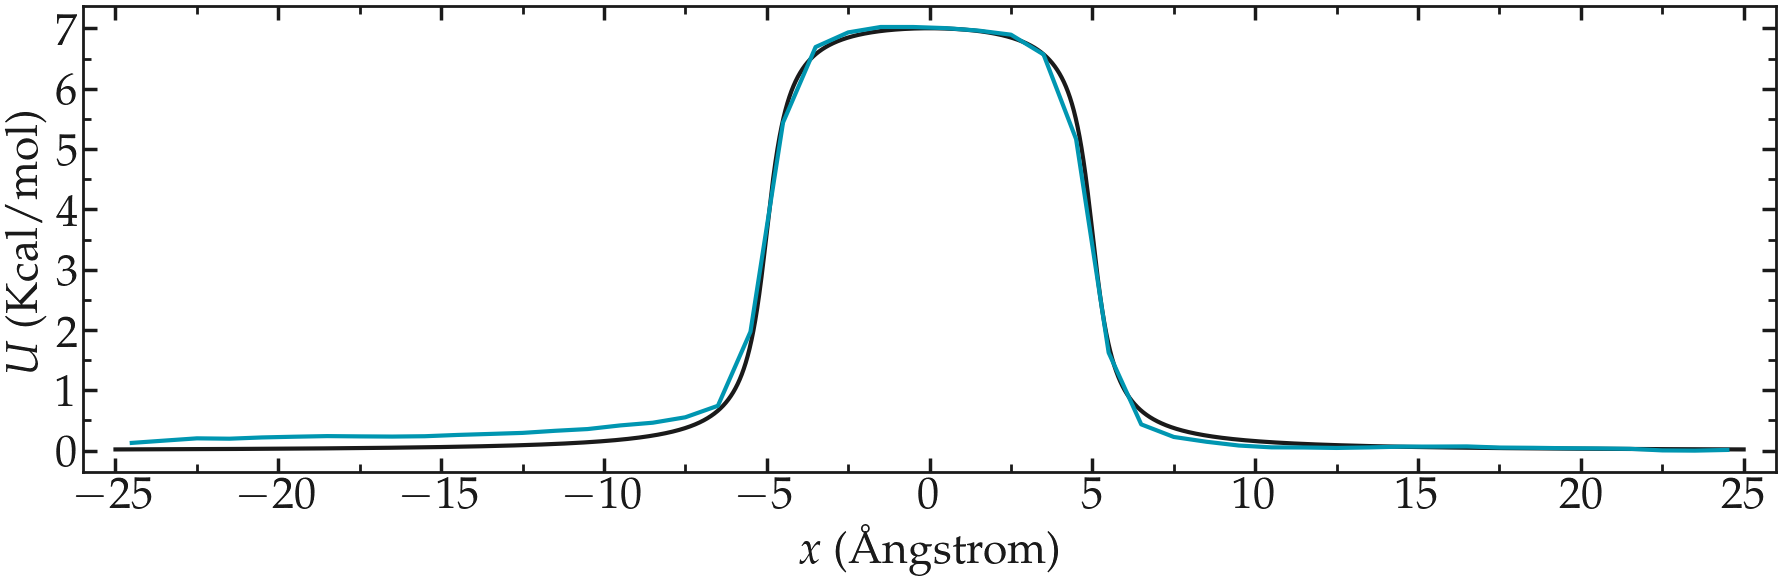
\includegraphics[width=\linewidth]{tutorials/level3/free-energy-calculation/freeenergy-light.png}
\end{figure}

We can see that the agreement is quite good despite the very short calculation time
and the very high value for the energy barrier. 

\subsection{Side note: on the choice of k}

\noindent As already stated, one difficult part of umbrella sampling is to choose the value of $k$.
Ideally, you want the biasing potential to be strong enough to force
the chosen atom to move along the axis, and you also want the
fluctuations of the atom position to be large enough to
have some overlap in the density probability of two
neighbor positions, like we have here with $k = 1.5$:

\begin{figure}
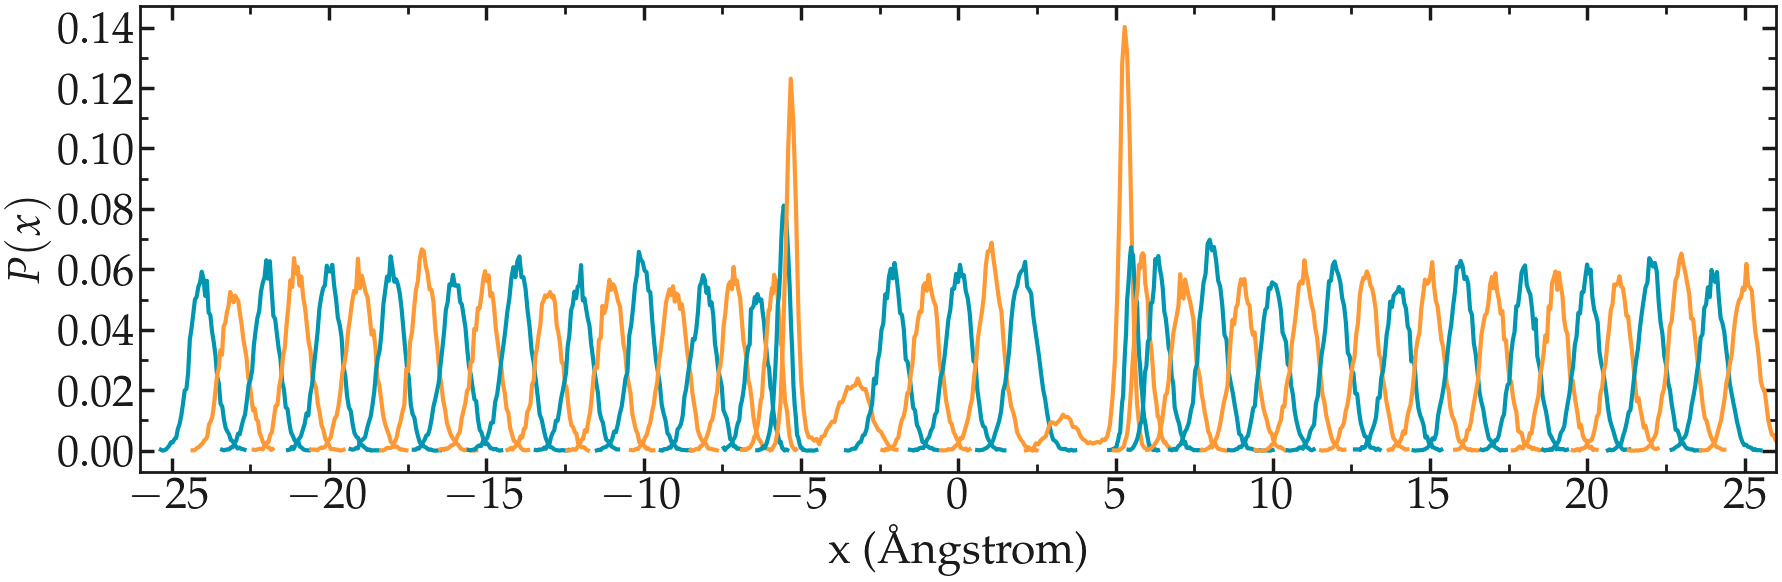
\includegraphics[width=\linewidth]{tutorials/level3/free-energy-calculation/overlap-light.png}
\end{figure}

If $k$ is too small, the biasing potential is too weak to force the particle to explores the 
region of interest, making it impossible to reconstruct the PMF:

\begin{figure}
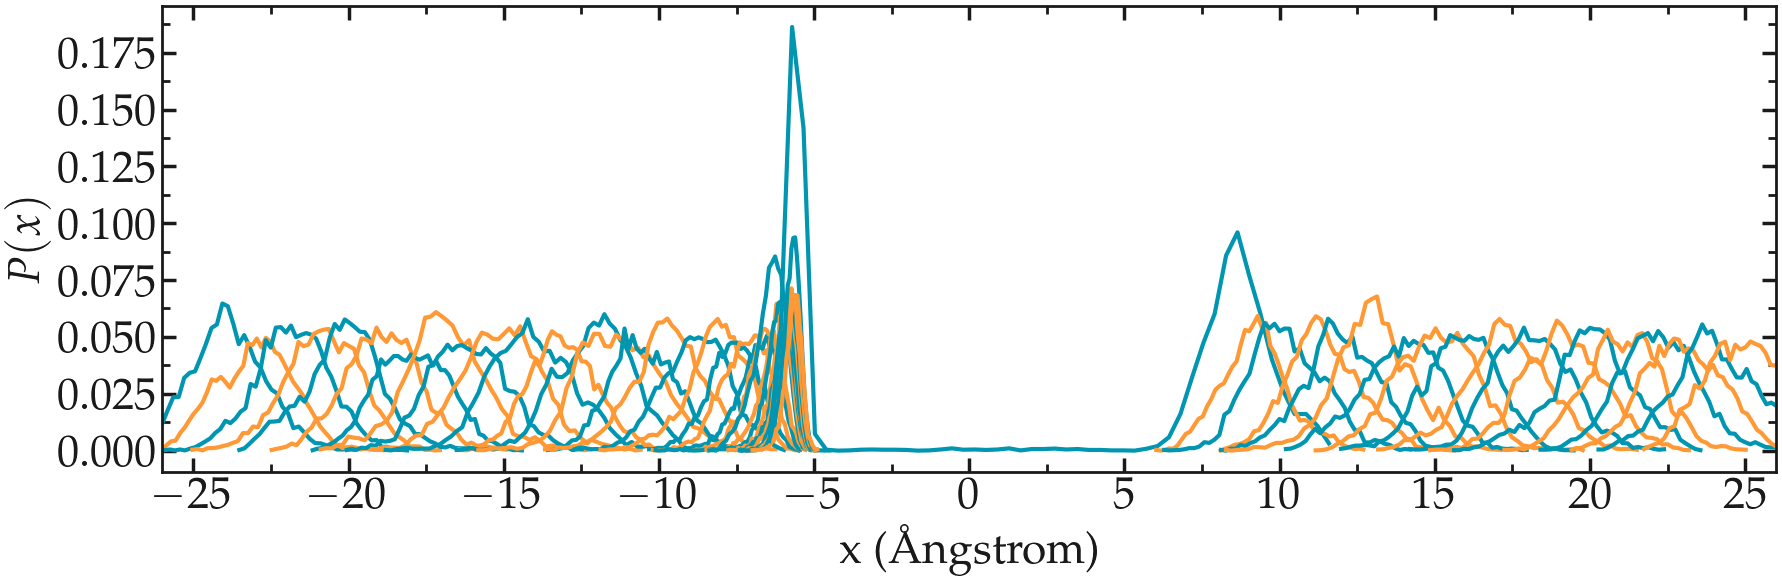
\includegraphics[width=\linewidth]{tutorials/level3/free-energy-calculation/overlap015-light.png}
\end{figure}

If $k$ is too large, the biasing potential is too large 
compared to the potential one want to probe, which reduces the 
sensitivity of the method. In that case, note the bad overlap between neighbor windows:

\begin{figure}
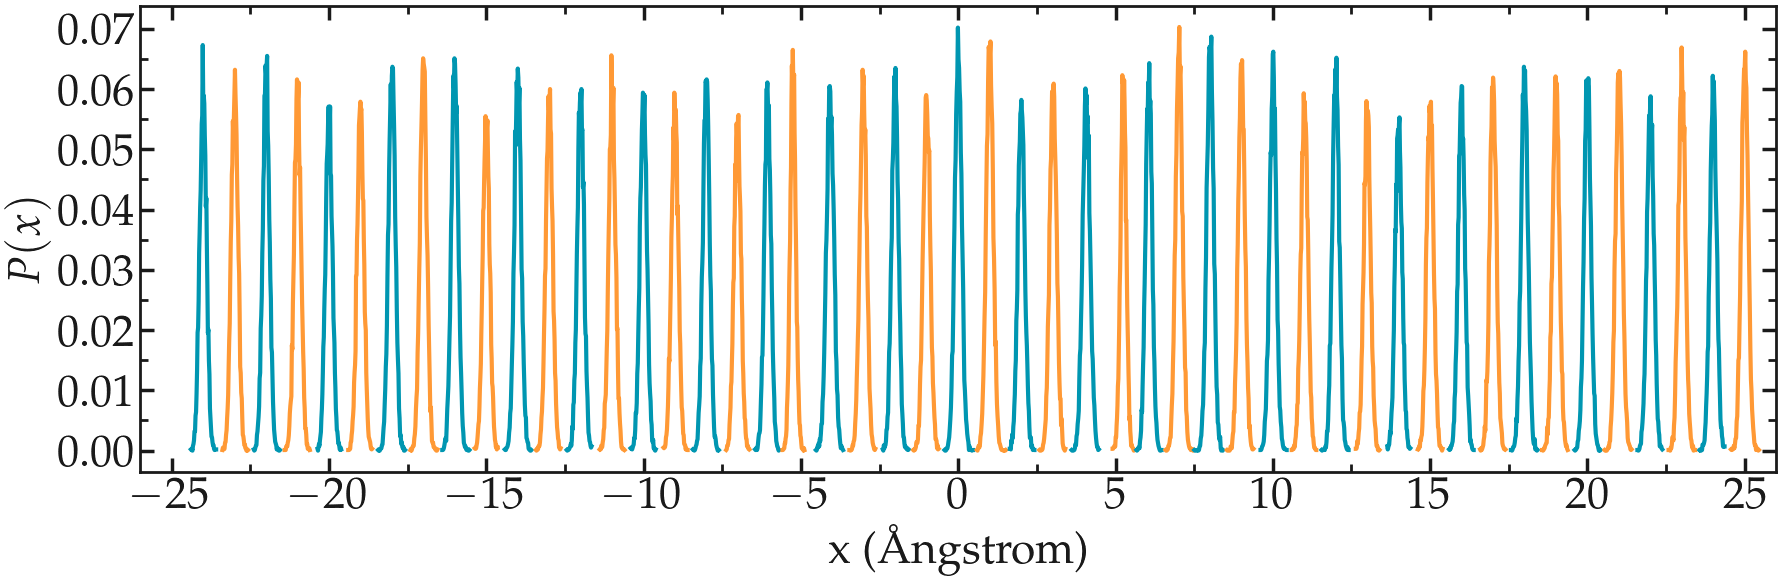
\includegraphics[width=\linewidth]{tutorials/level3/free-energy-calculation/overlap15-light.png}
\end{figure}

\section{Going further with exercises}

\noindent \subsection{The binary fluid that wont mix}

1 - Create the system\textit{}
Create a molecular simulation with two species of respective types 1 and 2.
Apply different potentials $U1$ and $U2$ on particles of types 1 and 2, respectively,
so that particles of type 1 are excluded from the center of the box, while at the same time particles
of type 2 are excluded from the rest of the box, as seen here:

\begin{figure}
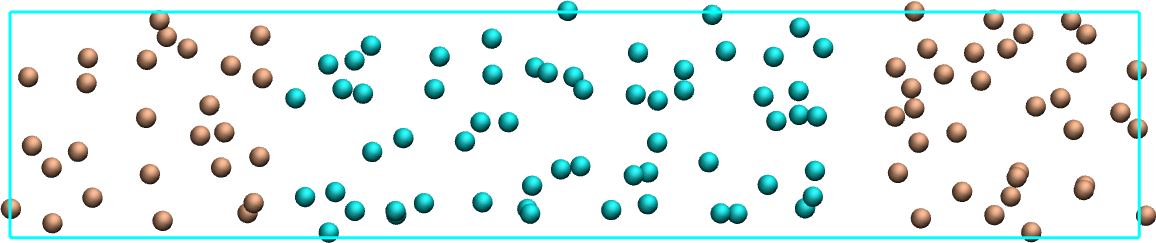
\includegraphics[width=\linewidth]{tutorials/level3/free-energy-calculation/exercice2-light.png}
\end{figure}

\begin{tcolorbox}[colback=mylightblue!5!white,colframe=mylightblue!75!black,title=Solution]

\begin{lcverbatim}

group t1 type 1
variable U1 atom ${U0}*atan((x+${x0})/${dlt})-${U0}*atan((x-${x0})/${dlt})
variable F1 atom ${U0}/((x-${x0})^2/${dlt}^2+1)/${dlt}-${U0}/((x+${x0})^2/${dlt}^2+1)/${dlt}
fix myadf1 t1 addforce v_F1 0.0 0.0 energy v_U1
fix_modify myadf1 energy yes
group t2 type 2
variable U2 atom -${U0}*atan((x+${x0})/${dlt})+${U0}*atan((x-${x0})/${dlt})
variable F2 atom -${U0}/((x-${x0})^2/${dlt}^2+1)/${dlt}+${U0}/((x+${x0})^2/${dlt}^2+1)/${dlt}
fix myadf2 t2 addforce v_F2 0.0 0.0 energy v_U2
fix_modify myadf2 energy yes
\end{lcverbatim}

\noindent \begin{lcverbatim}
mass * 39.95
pair_coeff * * ${epsilon} ${sigma}
\end{lcverbatim}

\noindent \end{tcolorbox}

2 - Measure the PMFs\textit{}
Using the same protocole as the one used in the tutorial (i.e. umbrella sampling with the wham algorithm),
extract the PMF for each particle type:

\begin{figure}
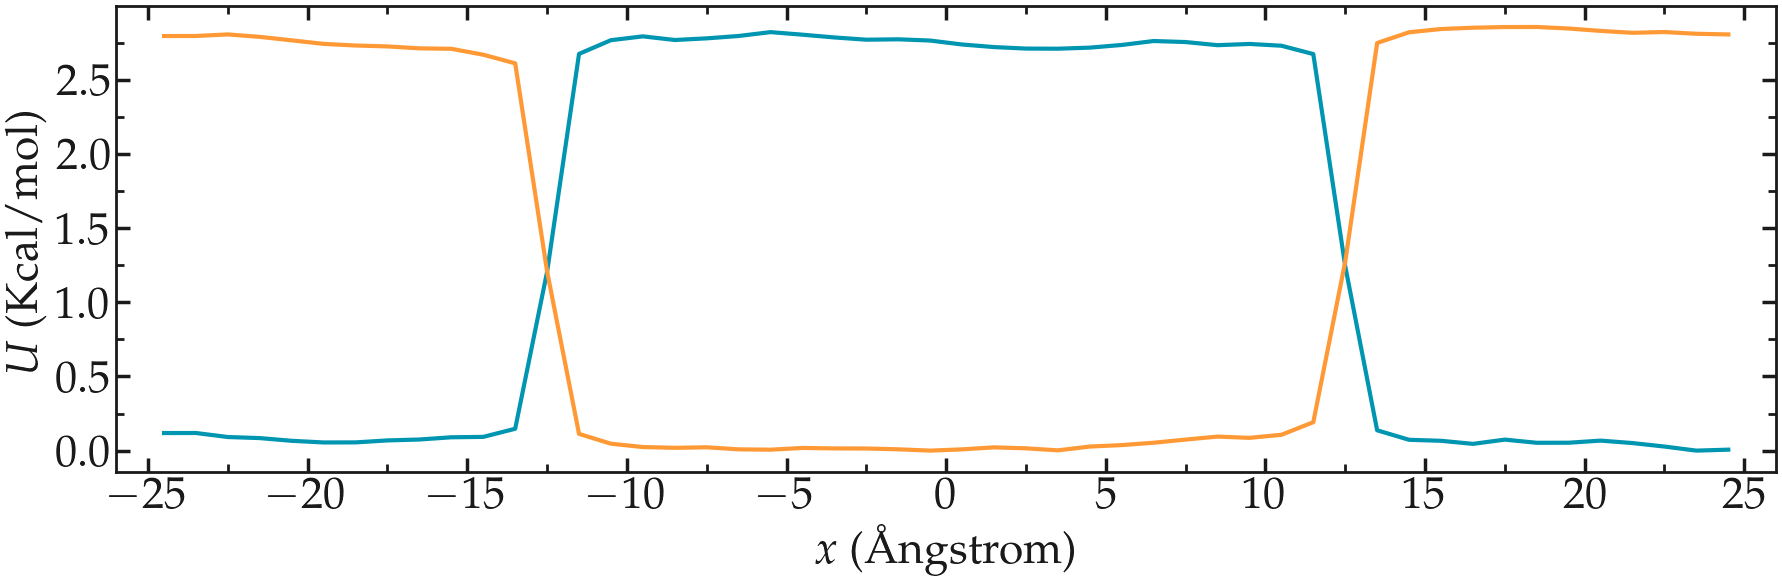
\includegraphics[width=\linewidth]{tutorials/level3/free-energy-calculation/exercice-binary-light.png}
\end{figure}

\subsection{Particles under convection}

\noindent Use a similar simulation as the one from the tutorial, with a repulsive potential in the center
of the box. Add a forcing to the particles and force them to flow in the $x$ direction.
Re-measure the potential in presence of the net convection of particles. You should see the 
potential getting tilted as a consequence of the additional force that makes it easier for 
the particles to cross the potential in one of the direction. The barrer will also 
reduced. 

\begin{figure}
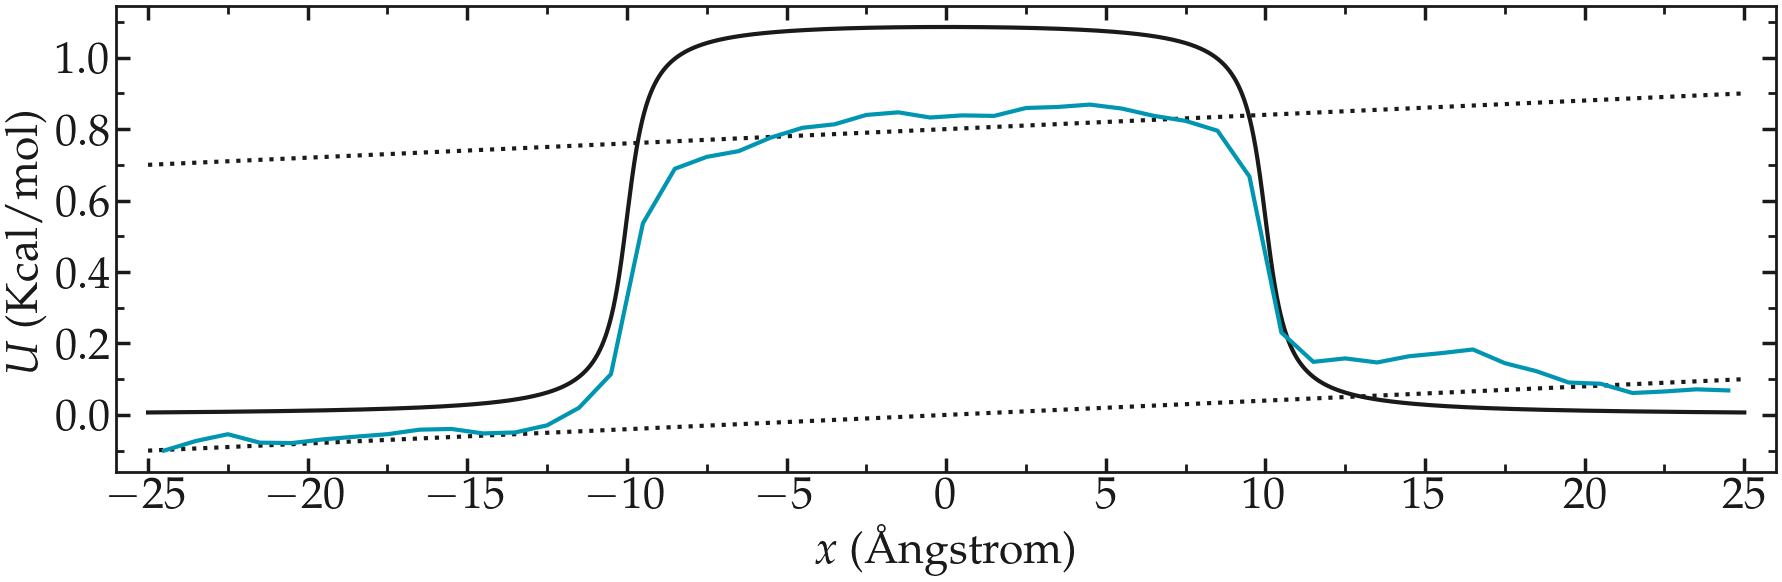
\includegraphics[width=\linewidth]{tutorials/level3/free-energy-calculation/exercice-convection-light.png}
\end{figure}

\begin{tcolorbox}[colback=mylightblue!5!white,colframe=mylightblue!75!black,title=Solution]

\begin{lcverbatim}
fix myconv all addforce 2e-6 0 0
\end{lcverbatim}

\noindent \end{tcolorbox}

\subsection{Surface adsorption of a molecule}

\noindent Apply umbrella sampling to calculate the free energy profile
of ethanol in the direction normal to a crystal solid surface (here made of sodium chloride). 
Find the \href{../../../../../inputs/level3/free-energy-calculation/Exercises/MoleculeAdsorption/system/}{topology files}, \href{../../../../../inputs/level3/free-energy-calculation/Exercises/MoleculeAdsorption/PARM.lammps}{parameter file}, and a \href{../../../../../inputs/level3/free-energy-calculation/Exercises/MoleculeAdsorption/input-minimalist.lammps}{minimal input file}.
The PMF normal to a wall indicates the free energy of adsorption, which is
calculated from the difference between the PMF far from the surface, and the 
PMF at the wall.

\begin{figure}
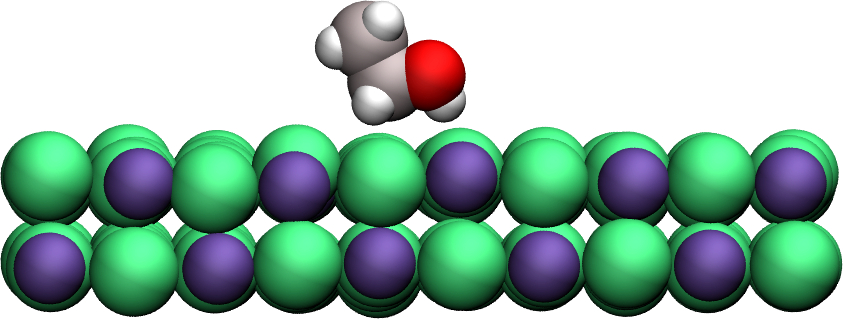
\includegraphics[width=\linewidth]{tutorials/level3/free-energy-calculation/ethanol-light.png}
\end{figure}

The PMF looks like that, with the position of the wall being near $x=0$.
The PMF mimina near the solid surface indicates the good affinity of the wall with 
the molecule.

\begin{figure}
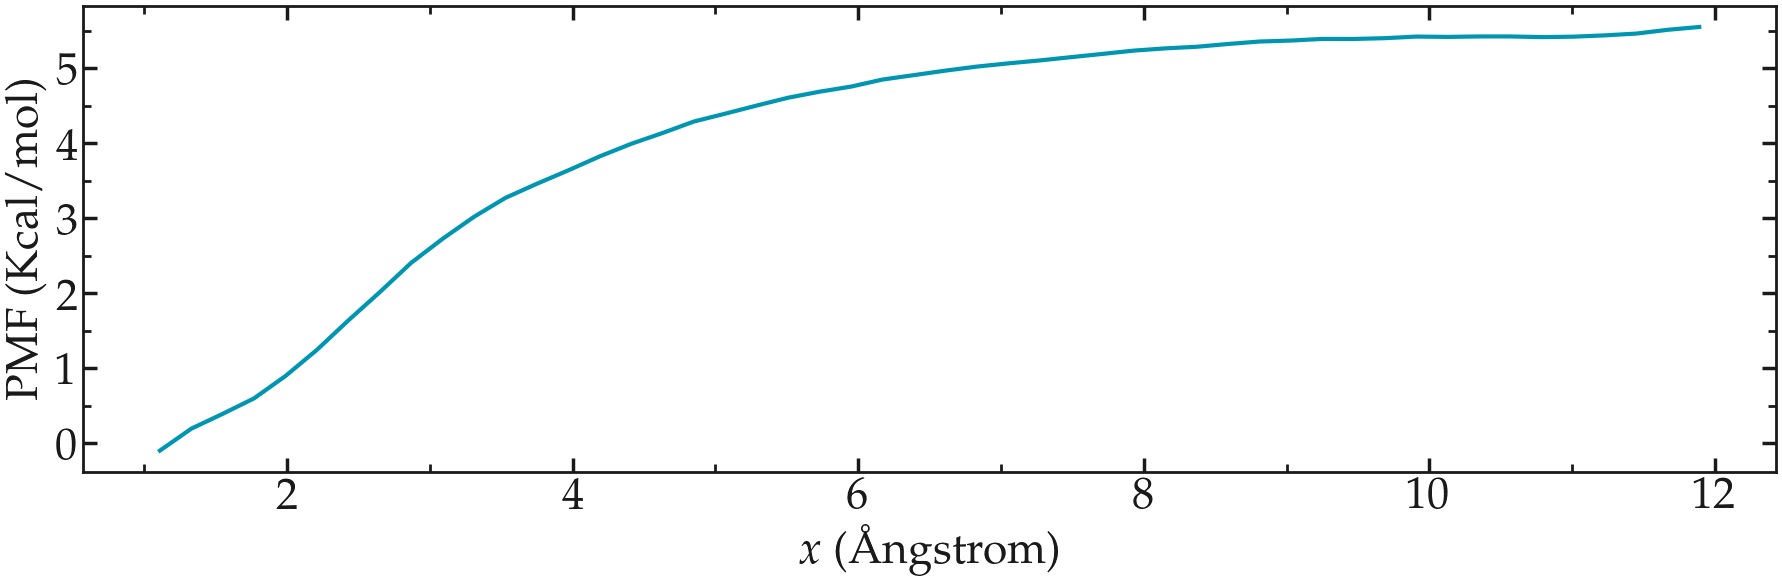
\includegraphics[width=\linewidth]{tutorials/level3/free-energy-calculation/exercice-ethanol-light.png}
\end{figure}

Alternatively to using ethanol, feel free to download the molecule of your choice, for 
instance from the  Automated Topology Builder (ATB). You will make your life simpler
by choosing one small molecule, like for instance CO2, a small alcohol, water, etc.

